% Options for packages loaded elsewhere
\PassOptionsToPackage{unicode}{hyperref}
\PassOptionsToPackage{hyphens}{url}
%
\documentclass[
  12pt,
]{article}
\usepackage{lmodern}
\usepackage{amssymb,amsmath}
\usepackage{ifxetex,ifluatex}
\ifnum 0\ifxetex 1\fi\ifluatex 1\fi=0 % if pdftex
  \usepackage[T1]{fontenc}
  \usepackage[utf8]{inputenc}
  \usepackage{textcomp} % provide euro and other symbols
\else % if luatex or xetex
  \usepackage{unicode-math}
  \defaultfontfeatures{Scale=MatchLowercase}
  \defaultfontfeatures[\rmfamily]{Ligatures=TeX,Scale=1}
  \setmainfont[]{Times New Roman}
\fi
% Use upquote if available, for straight quotes in verbatim environments
\IfFileExists{upquote.sty}{\usepackage{upquote}}{}
\IfFileExists{microtype.sty}{% use microtype if available
  \usepackage[]{microtype}
  \UseMicrotypeSet[protrusion]{basicmath} % disable protrusion for tt fonts
}{}
\makeatletter
\@ifundefined{KOMAClassName}{% if non-KOMA class
  \IfFileExists{parskip.sty}{%
    \usepackage{parskip}
  }{% else
    \setlength{\parindent}{0pt}
    \setlength{\parskip}{6pt plus 2pt minus 1pt}}
}{% if KOMA class
  \KOMAoptions{parskip=half}}
\makeatother
\usepackage{xcolor}
\IfFileExists{xurl.sty}{\usepackage{xurl}}{} % add URL line breaks if available
\IfFileExists{bookmark.sty}{\usepackage{bookmark}}{\usepackage{hyperref}}
\hypersetup{
  pdftitle={Dams in North Carolina: A Case Study of the Falls Lake Dam},
  pdfauthor={Cheney Gardner and Yingfan Zeng},
  hidelinks,
  pdfcreator={LaTeX via pandoc}}
\urlstyle{same} % disable monospaced font for URLs
\usepackage[margin=2.54cm]{geometry}
\usepackage{longtable,booktabs}
% Correct order of tables after \paragraph or \subparagraph
\usepackage{etoolbox}
\makeatletter
\patchcmd\longtable{\par}{\if@noskipsec\mbox{}\fi\par}{}{}
\makeatother
% Allow footnotes in longtable head/foot
\IfFileExists{footnotehyper.sty}{\usepackage{footnotehyper}}{\usepackage{footnote}}
\makesavenoteenv{longtable}
\usepackage{graphicx,grffile}
\makeatletter
\def\maxwidth{\ifdim\Gin@nat@width>\linewidth\linewidth\else\Gin@nat@width\fi}
\def\maxheight{\ifdim\Gin@nat@height>\textheight\textheight\else\Gin@nat@height\fi}
\makeatother
% Scale images if necessary, so that they will not overflow the page
% margins by default, and it is still possible to overwrite the defaults
% using explicit options in \includegraphics[width, height, ...]{}
\setkeys{Gin}{width=\maxwidth,height=\maxheight,keepaspectratio}
% Set default figure placement to htbp
\makeatletter
\def\fps@figure{htbp}
\makeatother
\setlength{\emergencystretch}{3em} % prevent overfull lines
\providecommand{\tightlist}{%
  \setlength{\itemsep}{0pt}\setlength{\parskip}{0pt}}
\setcounter{secnumdepth}{5}

\title{Dams in North Carolina: A Case Study of the Falls Lake Dam}
\usepackage{etoolbox}
\makeatletter
\providecommand{\subtitle}[1]{% add subtitle to \maketitle
  \apptocmd{\@title}{\par {\large #1 \par}}{}{}
}
\makeatother
\subtitle{\url{https://github.com/cheneygardner/ENV872-Final-Project.git}}
\author{Cheney Gardner and Yingfan Zeng}
\date{}

\begin{document}
\maketitle

\hypertarget{rationale-and-research-questions}{%
\section{Rationale and Research
Questions}\label{rationale-and-research-questions}}

According to the Army Corps of Engineers' National Inventory of Dams,
North Carolina has 3191 dams, including the Falls Lake Dam. The Falls
Lake Dam was completed in 1981 to manage the flow of the Neuse River.
Flood control dams remove high flows but can have anthropogenic impacts
on the ecological needs of many aquatic species. For example, if a fish
species has evolved to be triggered to spawn by high flows, a flood
control dam may reduce future reproduction.

Over the past three decades, a series of smaller dams downstream on the
Neuse have been removed, and the Neuse River now flows freely from Falls
Lake to the Pamlico Sound for the first time in 100 years. Research has
shown that the removal of these downstream dams has positive ecological
effects on fish migration (Raabe and Hightower, 2014). It is thought
that the migration was potentially triggered by changes in the river
flow as larger flows reduced salinity in estuaries and triggered the
fish to migrate upstream.

In order to further explore the impact of a dam on the hydrological
environment, we chose the Falls Lake Dam as a case study for a more
in-depth analysis. Knowing whether there was a change in streamflow, and
what type of change, is useful information for ecologists studying the
impact of dams on the habitat of species like shad.

Research Question:

\begin{itemize}
\tightlist
\item
  \emph{Was there any change in discharge before and after the
  construction of the Falls Lake Dam and, if so, are there trends?}
\end{itemize}

\newpage

\hypertarget{dataset-information}{%
\section{Dataset Information}\label{dataset-information}}

\hypertarget{dam-removal-spatial-data}{%
\subsection{Dam Removal Spatial Data}\label{dam-removal-spatial-data}}

The Falls Lake Dam has received increased interest since the removal of
downstream dams, most recently the Milburnie Dam in 2017. To visualize
the downstream dams removed on the Neuse River and others around the
state, we used categorical and spatial data from the American Rivers Dam
Removal Database. The database contains 1,775 entries dating back to
1912, but our sample size was small, as North Carolina contains only 36
removed dams.

We database includes all known dam removals in the U.S. from 1916-2016.
(Note: It is nearly impossible to determine the exact number or dams
removed or when they were constructed because many don't meet the US
Army Corps of Engineers' National Inventory of Dams.) American Rivers
defines a dam as removed if: \emph{a significant portion of the dam must
have been removed for the full height of the dam, such that ecological
function, natural river flow and fish passage can be restored at the
site.}

The dataset contained American Rivers-specific ID, National ID number,
Dam Name, Year Removed, Latitude, Longitude, City and/or County, River,
HUC8, State, Dam Height, Dam Length, Owner, Year Built, Original Use,
Type of Material, Miles Restored and River Miles Reported. For the
purposes of our analysis, we selected only entries from North Carolina
and wrangled only the Dam Name, Year Removed, City and/or County, River,
HUC8 and geometry columns. Two unnamed dams in North Carolina, AR-ID
NC-010 and NC-029, did not have any spatial data, which was critical to
our exploratory analysis, so they had to be removed.

\hypertarget{discharge-data}{%
\subsection{Discharge Data}\label{discharge-data}}

To evaluate the change in discharge before and after the construction of
the Falls Lake Dam, we used daily mean discharge data from four USGS
streamflow gages on the Neuse River. The gage data was downloaded from
the USGS National Water Information System.

The date ranges of discharge data available is dependent on the dates in
which the gage has been in use. For example, daily mean discharge data
is available from Gage \#02087183 from 1970 to 2020. Due to seasonality,
we only examined data from full years, ending in 2020. The spatial gage
data was also retrieved from the USGS National Water Information System.

Gage Station Name \textbar{} Gage ID\\
\_\_\_\_\_\_\_\_\_\_\_\_\_\_\_\_\_\_\_ \textbar{}
\_\_\_\_\_\_\_\_\_\_\_\\
Falls Lake \textbar{} 02087183\\
Clayton \textbar{} 02087500\\
Goldsboro \textbar{} 02089000\\
Kinston \textbar{} 02089500

\hypertarget{data-wrangling}{%
\subsection{Data Wrangling}\label{data-wrangling}}

The discharge data was wrangled before further analysis. To analyze the
data from each gage, we dropped NA data, changed column names and
mutated the date columns to the date format. Then, we combined data from
all the four gages to produce a total dataset. We also aggregated daily
discharge data by gage to generate another total dataset to prepare for
following analysis.

\newpage

\hypertarget{exploratory-analysis}{%
\section{Exploratory Analysis}\label{exploratory-analysis}}

To understand the spatial context of the four gage sites, we mapped the
gage sites, the Falls Lake Dam and the HUC 8 watershed boundaries. (The
HUC 8 hydrologic units were used on both maps because they were
available and relevant for the gage data and dam removal datasets.)
Using Leaflet, we included information on the USGS Station, County and
HUC 8 Subbasin of the gage station, which could be retrieved when the
user interacted with the map. We built functions that allowed us to
customize the coloring and made sure important information, like the
title, did not move when zooming in or out. (We included PNG versions of
the maps in our report. The original HTML code can be found on our
github repository Code folder.)

Falls Lake Dam and Gage Station Locations used for Discharge Analysis

\begin{figure}
\centering
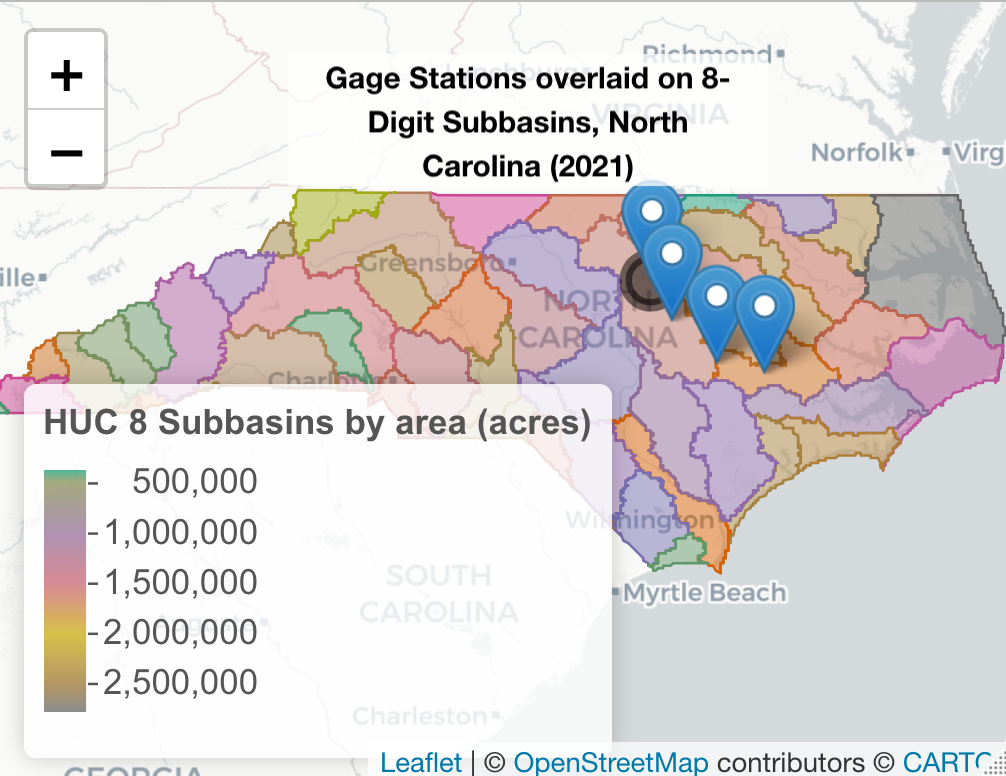
\includegraphics{"./Output/gage.station.png"}
\caption{Gage Stations Analyzed for Falls Lake Dam}
\end{figure}

\hypertarget{dam-removal-patterns}{%
\subsection{Dam Removal Patterns}\label{dam-removal-patterns}}

To visualize the downstream dams removed on the Neuse River and others
around the state, we wrangled American Rivers Dam Removal Database to
only include information from North Carolina. Then we filtered for the
information relevant to our spatial analysis: latitude/longitude, dam
name, removal year and HUC 8 watershed basin. When we conducted our
analysis of discharge data from the different gage sites, these maps
allowed us to easily determine whether there were spatial patterns to
changes in discharge. The maps also allowed us to quickly determine
which dams on the Neuse had previously been removed, as well as what
other dams in the same HUC watershed.

Dams Removed in North Carolina since 1916, including on Neuse River

\begin{figure}
\centering
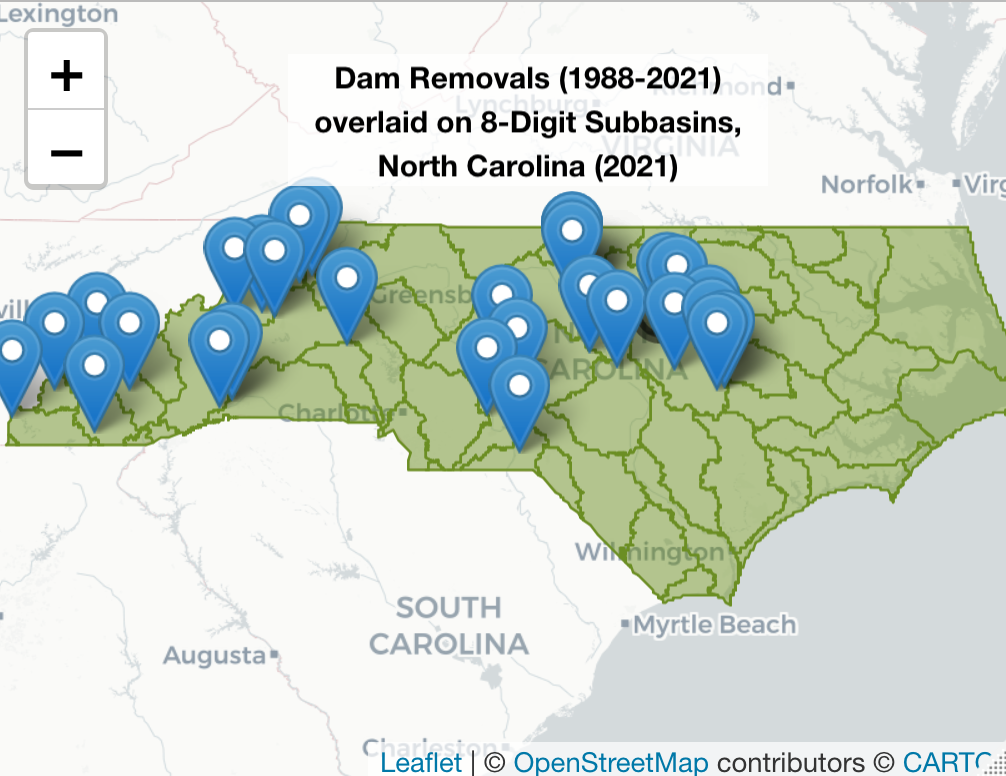
\includegraphics{"./Output/dam.removal.map.png"}
\caption{Dams Removed in North Carolina since 1916}
\end{figure}

\hypertarget{initial-data-wrangling}{%
\subsection{Initial Data Wrangling}\label{initial-data-wrangling}}

In order to have a preliminary basic understanding of the discharge data
at the four gages, we plotted the annual average discharge at the four
gages by time. The year the Falls Lake Dam was completed, 1981, is
marked with a vertical line. As visible in our map, the order of gage
locations the nearest to the farthest distance from the Falls Lake Dam
is Falls Lake, Clayton, Goldsboro, Kinston. Discharge at the two closer
gages is significantly lower than that at the two farther gages. The
flow changes before and after the dam was built are not obvious in this
figure.

\begin{verbatim}
## Warning: Removed 1 row(s) containing missing values (geom_path).
\end{verbatim}

\begin{figure}

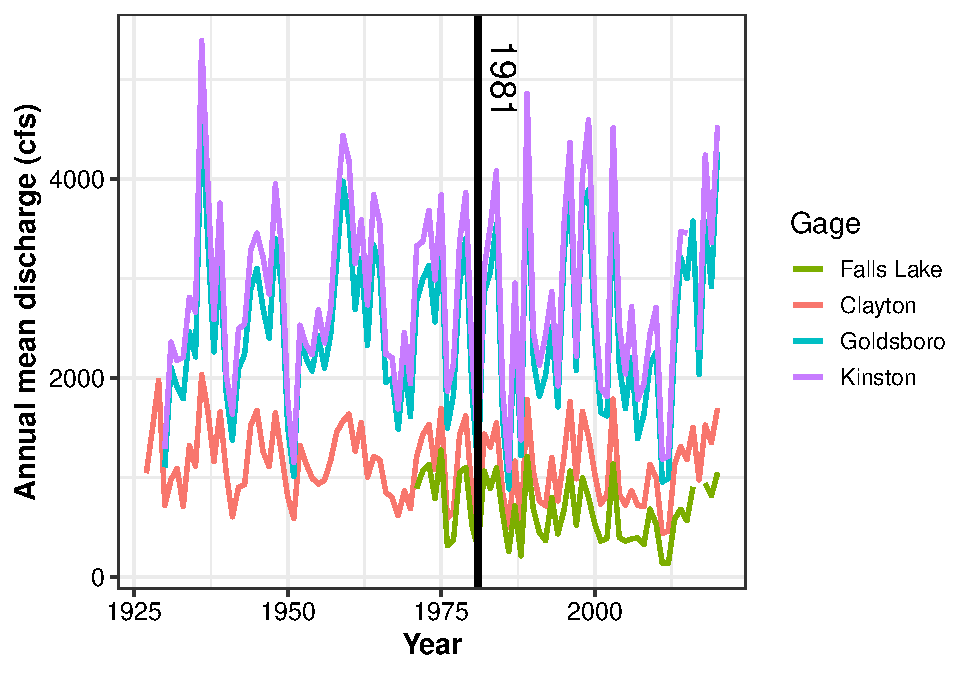
\includegraphics{Gardner_Zeng_pdf_output_files/figure-latex/Plot annual mean discharge-1} \hfill{}

\caption{Annual Average Discharge at 4 Gages}\label{fig:Plot annual mean discharge}
\end{figure}

\hypertarget{analysis}{%
\section{Analysis}\label{analysis}}

\hypertarget{hydrological-impacts-of-the-construction-of-falls-lake-dam}{%
\subsection{Hydrological impacts of the construction of Falls Lake
Dam}\label{hydrological-impacts-of-the-construction-of-falls-lake-dam}}

The first step to explore the changes in the discharge of the Neuse
River downstream of the Falls Lake Dam was to conduct a time series
analysis. From the time series analysis results (Figure 3-6), all the
four gages showed clear seasonal cycles, but the general trends remained
vague.

\begin{figure}

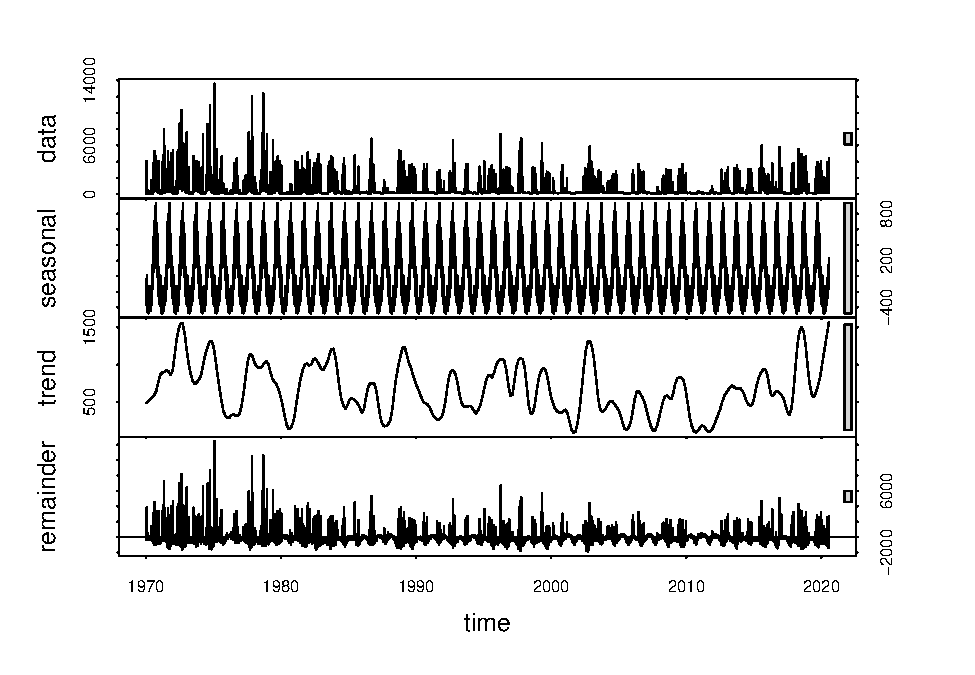
\includegraphics{Gardner_Zeng_pdf_output_files/figure-latex/Time series Falls Lake-1} \hfill{}

\caption{Time Series Analysis on the discharge data at the Falls Lake gage}\label{fig:Time series Falls Lake}
\end{figure}

\begin{figure}

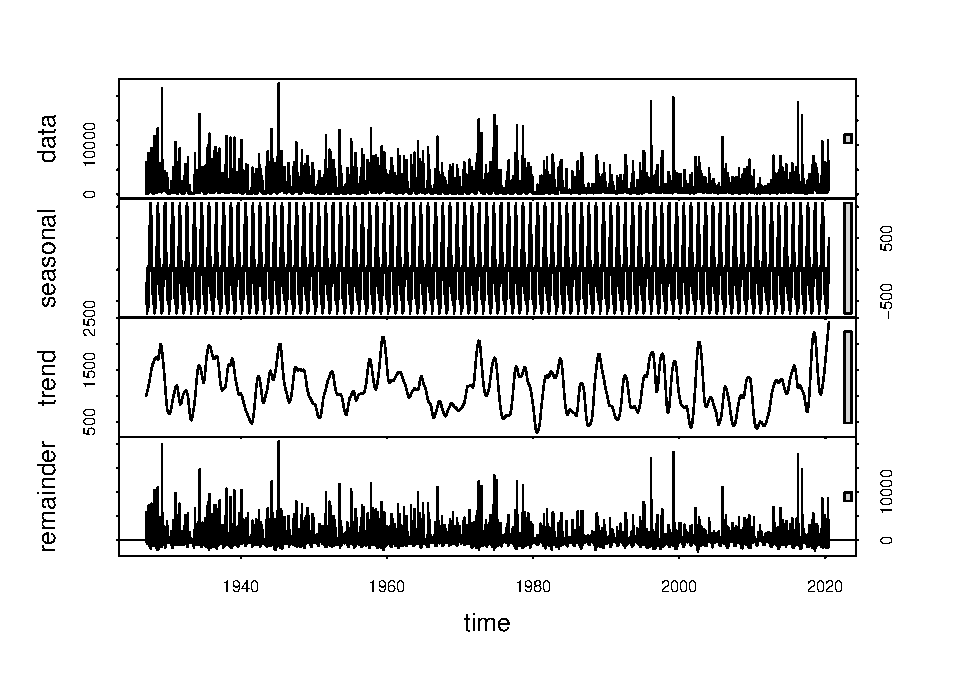
\includegraphics{Gardner_Zeng_pdf_output_files/figure-latex/Time series Clayton-1} \hfill{}

\caption{Time Series Analysis on the discharge data at the Clayton gage}\label{fig:Time series Clayton}
\end{figure}

\begin{figure}

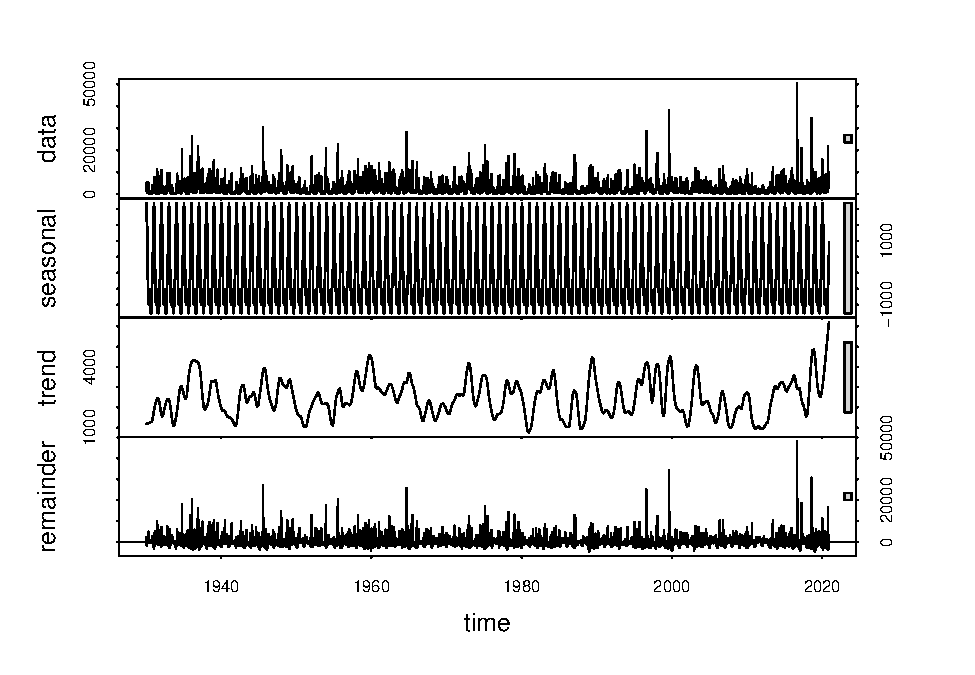
\includegraphics{Gardner_Zeng_pdf_output_files/figure-latex/Time series Goldsboro-1} \hfill{}

\caption{Time Series Analysis on the discharge data at the Goldsboro gage}\label{fig:Time series Goldsboro}
\end{figure}

\begin{figure}

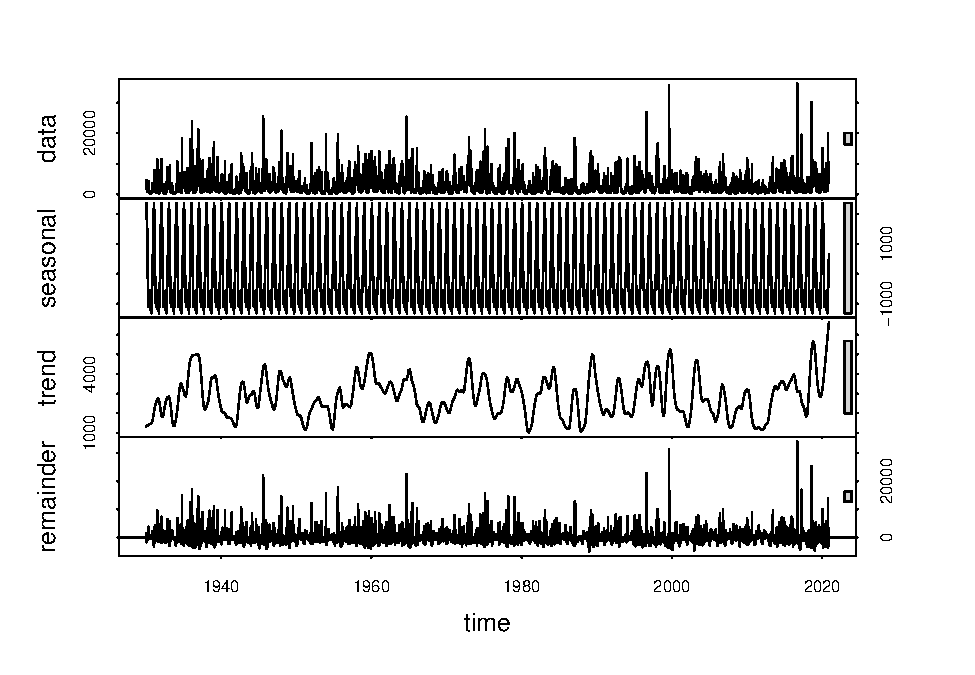
\includegraphics{Gardner_Zeng_pdf_output_files/figure-latex/Time series Kinston-1} \hfill{}

\caption{Time Series Analysis on the discharge data at the Kinston gage}\label{fig:Time series Kinston}
\end{figure}

To further explore the trend of discharge over time, we performed a
linear regression analysis on the data (Figure 7-10). Discharge at Falls
Lake and Clayton gages decreased with a negative slope, while the slopes
of Goldsboro and Kinston were slightly positive. However, the R square
of all the four regrssion was small, which meant the fit of the model
was poor for flow data with large fluctuations.

\begin{figure}

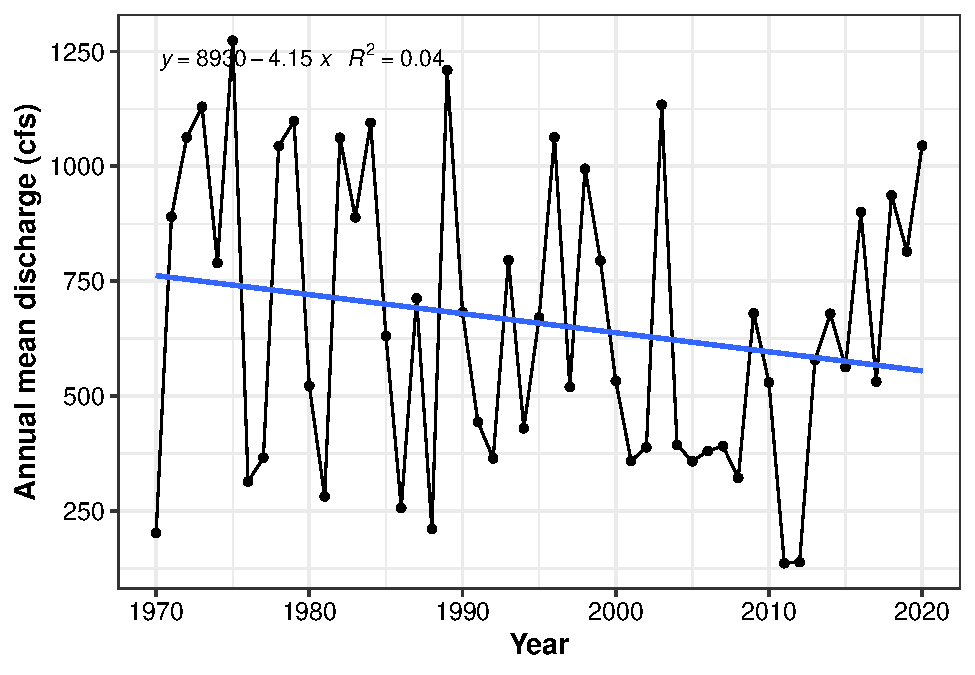
\includegraphics{Gardner_Zeng_pdf_output_files/figure-latex/GLM Falls Lake-1} \hfill{}

\caption{Generalized linear regression on the annual discharge data at the Falls Lake gage}\label{fig:GLM Falls Lake}
\end{figure}

\begin{figure}

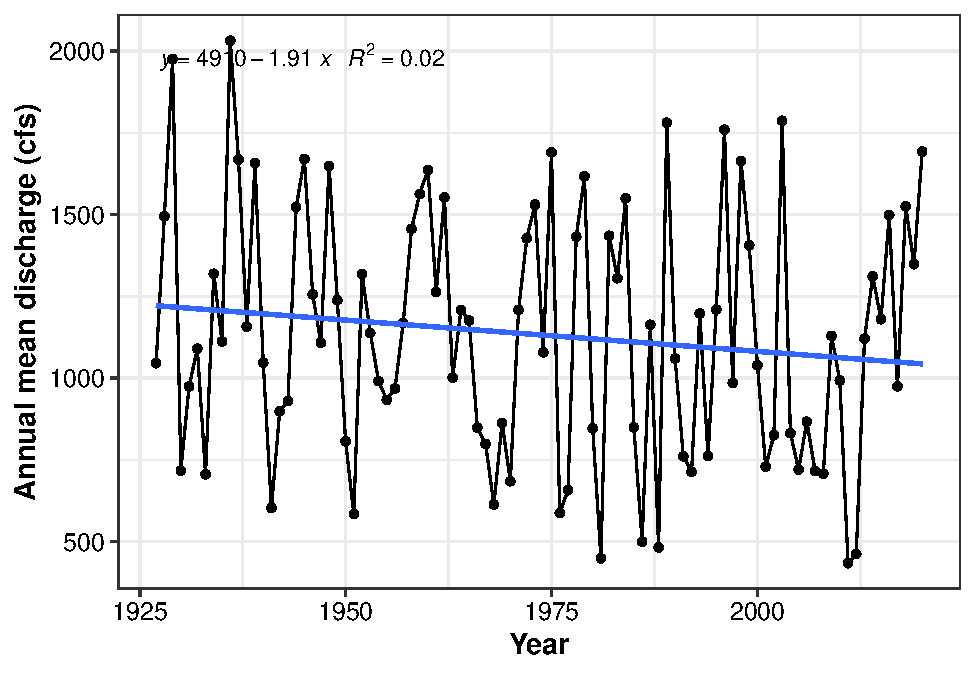
\includegraphics{Gardner_Zeng_pdf_output_files/figure-latex/GLM Clayton-1} \hfill{}

\caption{Generalized linear regression on the annual discharge data at the Clayton gage}\label{fig:GLM Clayton}
\end{figure}

\begin{figure}

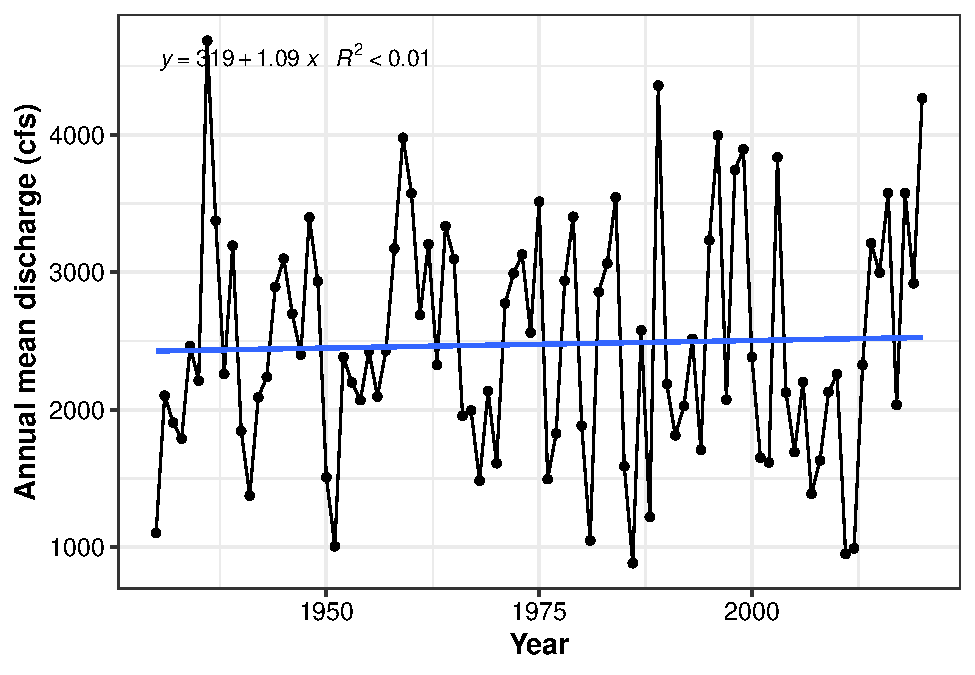
\includegraphics{Gardner_Zeng_pdf_output_files/figure-latex/GLM Goldsboro-1} \hfill{}

\caption{Generalized linear regression on the annual discharge data at the Goldsboro gage}\label{fig:GLM Goldsboro}
\end{figure}

\begin{figure}

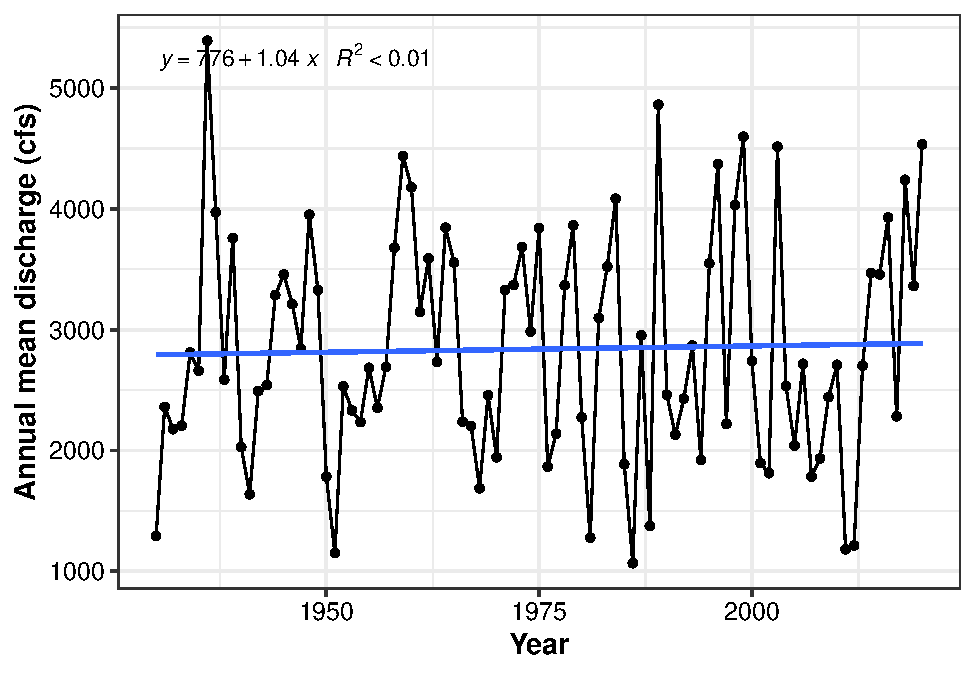
\includegraphics{Gardner_Zeng_pdf_output_files/figure-latex/GLM Kinston-1} \hfill{}

\caption{Generalized linear regression on the annual discharge data at the Kinston gage}\label{fig:GLM Kinston}
\end{figure}

Finally, we conducted a t-test for pre- and post-dam average discharge
for each site. Given that the Falls Lake Dam was built between 1978 and
1981, the pre-dam period of each gage is defined as from the beginning
of records to December 31st, 1977, while the post-dam period is from
January 1st, 1982 to December 31st, 2020. The results of the t-test are
shown in Table 2. Discharge at the Falls Lake gage and the Clayton gage
significantly decreased after the dam construction, with a p-value less
than 0.05. And the other two gages have little change in discharge
before and after the dam building with high p values.

\begin{longtable}[]{@{}lrrr@{}}
\caption{Results of the t-test on discharge before and after the
construction of the Falls Lake Dam}\tabularnewline
\toprule
& Pre-dam mean discharge & Post-dam mean discharge & P
value\tabularnewline
\midrule
\endfirsthead
\toprule
& Pre-dam mean discharge & Post-dam mean discharge & P
value\tabularnewline
\midrule
\endhead
Falls Lake & 789.0616 & 631.2978 & 0.0000000\tabularnewline
Clayton & 1170.6212 & 1089.0022 & 0.0000008\tabularnewline
Goldsboro & 2484.4243 & 2488.1184 & 0.9080408\tabularnewline
Kinston & 2851.8914 & 2843.3724 & 0.7992888\tabularnewline
\bottomrule
\end{longtable}

\newpage

\hypertarget{summary-and-conclusions}{%
\section{Summary and Conclusions}\label{summary-and-conclusions}}

、 While the number of Dams being removed in North Carolina has
increased in recent years, the hydrological impacts of dams on rivers
remains unclear. Taking the Falls Lake Dam for a closer study on its
hydrological impacts, we analyzed the changes of downstream discharge
before and after its construction After the construction of the Falls
Lake Dam, the discharge at the two downstream gages closest to the dam
(Falls Lake and Clayton) decreased, while the discharge of two farther
gages (Goldsboro and Kinston) had no obvious change. It may be because
longer distance and annexed tributaries weaken the dam's influence on
the discharge at these two gages. We can conclude that the Falls Lake
Dam reduced the discharge of a river within a certain distance. This
information is valuable for the hydrological effects of other dams in
North Carolina, as well as for dam management and future dam removal.

\newpage

\hypertarget{references}{%
\subsection{References}\label{references}}

Raabe, J. K., and Hightower, J. E. (2014). Assessing distribution of
migratory fishes and connectivity following complete and partial dam
removals in a North Carolina river. \emph{North American Journal of
Fisheries Management}, 34(5), 955-969.

Rivers, American (2017): American Rivers Dam Removal Database. figshare.
\url{https://doi.org/10.6084/m9.figshare.5234068.v2}

U.S. Geological Survey. (2016), National Water Information System data
available on the World Wide Web (USGS Water Data for the Nation),
accessed at URL \url{http://waterdata.usgs.gov/nwis/}

\end{document}
